\documentclass[12pt, a4paper]{article}
\usepackage{fancyhdr}
\pagestyle{fancy}
\lhead{jcl187}
\chead{Allan Nielsen}
\rhead{}
\usepackage[margin=1.0 in]{geometry}
\addtolength{\topmargin}{.25in}
\usepackage[utf8]{inputenc}  
\usepackage{amsmath}
\usepackage[danish]{babel}
\usepackage{calc}
\usepackage{array}
\usepackage{listings}
\usepackage{color}
\definecolor{mygreen}{rgb}{0,0.6,0}
\definecolor{mygray}{rgb}{0.5,0.5,0.5}
\definecolor{mymauve}{rgb}{0.58,0,0.82}
\lstset{ %
  backgroundcolor=\color{white},   % choose the background color; you must add \usepackage{color} or \usepackage{xcolor}
  basicstyle=\footnotesize,        % the size of the fonts that are used for the code
  breakatwhitespace=false,         % sets if automatic breaks should only happen at whitespace
  breaklines=true,                 % sets automatic line breaking
  captionpos=b,                    % sets the caption-position to bottom
  commentstyle=\color{mygreen},    % comment style
  deletekeywords={...},            % if you want to delete keywords from the given language
  escapeinside={\%*}{*)},          % if you want to add LaTeX within your code
  extendedchars=\true,              % lets you use non-ASCII characters; for 8-bits encodings only, does not work with UTF-8
  frame=single,                    % adds a frame around the code
  keepspaces=true,                 % keeps spaces in text, useful for keeping indentation of code (possibly needs columns=flexible)
  keywordstyle=\color{blue},       % keyword style
  language=Octave,                 % the language of the code
  morekeywords={*,...},            % if you want to add more keywords to the set
  numbers=left,                    % where to put the line-numbers; possible values are (none, left, right)
  numbersep=5pt,                   % how far the line-numbers are from the code
  numberstyle=\tiny\color{mygray}, % the style that is used for the line-numbers
  rulecolor=\color{black},         % if not set, the frame-color may be changed on line-breaks within not-black text (e.g. comments (green here))
  showspaces=false,                % show spaces everywhere adding particular underscores; it overrides 'showstringspaces'
  showstringspaces=false,          % underline spaces within strings only
  showtabs=false,                  % show tabs within strings adding particular underscores
  stepnumber=2,                    % the step between two line-numbers. If it's 1, each line will be numbered
  stringstyle=\color{blue},     % string literal style
  tabsize=2,                       % sets default tabsize to 2 spaces
  title=\lstname,                   % show the filename of files included with \lstinputlisting; also try caption instead of title
  inputencoding=ansinew
}
\lstset{literate=%
{æ}{{\ae}}1
{å}{{\aa}}1
{ø}{{\o}}1
{Æ}{{\AE}}1
{Å}{{\AA}}1
{Ø}{{\O}}1
{Ö}{{\"O}}1
{á}{{\'a}}1
}
\usepackage{amssymb}
%\usepackage{tikz}
\usepackage{graphicx}
\newcommand{\HRule}{\rule{\linewidth}{0.5mm}}
\usepackage{hyperref}
\newcommand{\Green}{\tikz\draw[green,fill=green] (0,0) circle (1 ex);}
\newcommand{\Lime }{\tikz\draw[brown,fill=brown] (0,0) circle (1 ex);}
\newcommand{\Blue}{\tikz\draw[blue,fill=blue] (0,0) circle (1 ex);}
\newcommand{\Yellow}{\tikz\draw[yellow,fill=yellow] (0,0) circle (1 ex);}
\newcommand{\Red}{\tikz\draw[red,fill=red] (0,0) circle (1 ex);}
\renewcommand*\contentsname{Indholdsfortegnelse}
%\usepackage{cleveref}

%\crefformat{footnote}{#2\footnotemark[#1]#3}

\setlength\parindent{0pt}		% noindent through whole document
\usepackage[parfill]{parskip}	% extra linebreak on new paragraph
\begin{document}
\section*{(b)}
Vi får følgende graf af $u(x,t)|t=10$\\
\begin{figure}[h!]
	\centering
	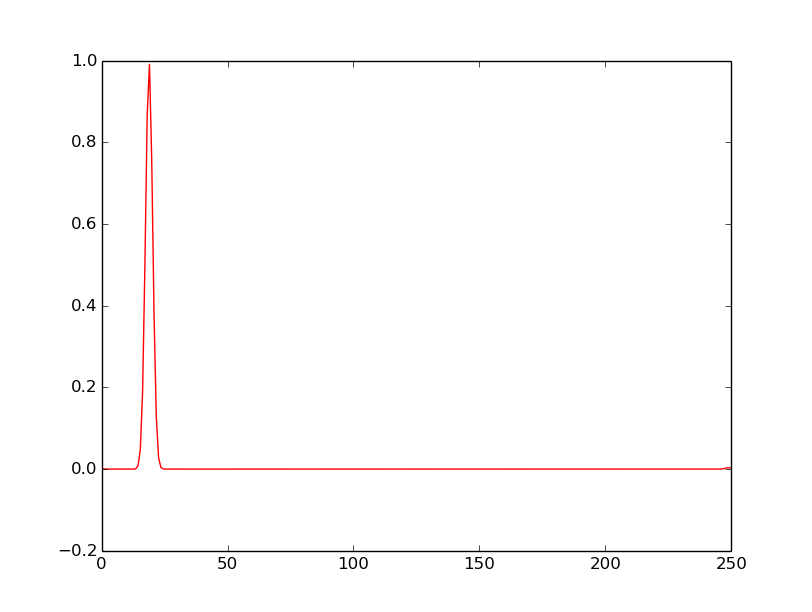
\includegraphics[scale=0.5]{die_welle2.png}\\
	\caption{for t=10}
\end{figure}
Vi får følgende graf af $u(x,t)|t=150$\\
\begin{figure}[h!]
	\centering
	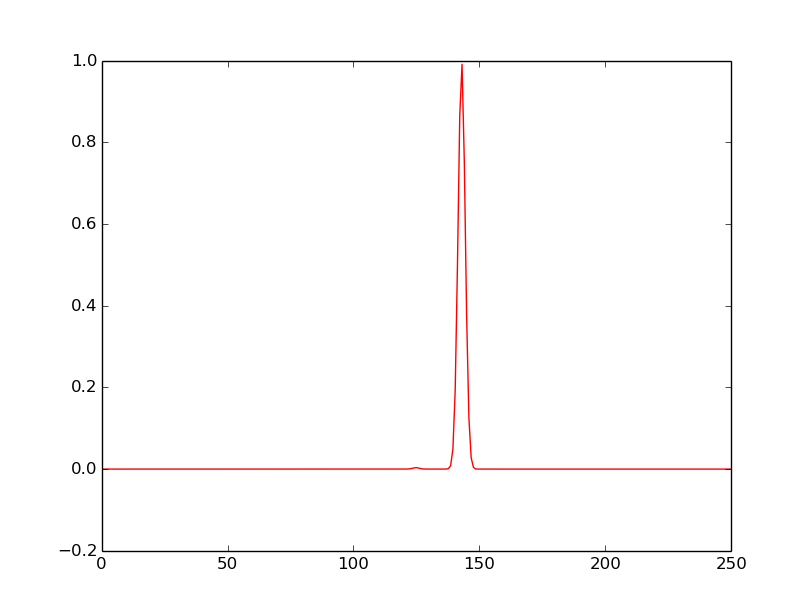
\includegraphics[scale=0.5]{die_welle3.png}\\
	\caption{for t=150}
\end{figure}\section*{(c)}
Når k ændres, får vi flere tispunkter for bølgen, idet at den ikke beregnes for alle heltal melem 0 og t, men for alle tal mellem 0 og t, med en skridt længde på k.\\
Når h ændres, 
Når vi sætter $c=1\ og\ l=250$ er bølgen netop $l$ om at om at komme en omgang rundt på stadion. Ihvertfald hvis vi skal gå ud fra figur\\
Figuren viser alle t til $l-1$ (dog er der nul-indexering), så $t=248$. Det ses at det sidste tidpunkt mangler og at der er en "hvid" bølge der hvor den kommer til at være.\\
\begin{figure}[h!]
	\centering
	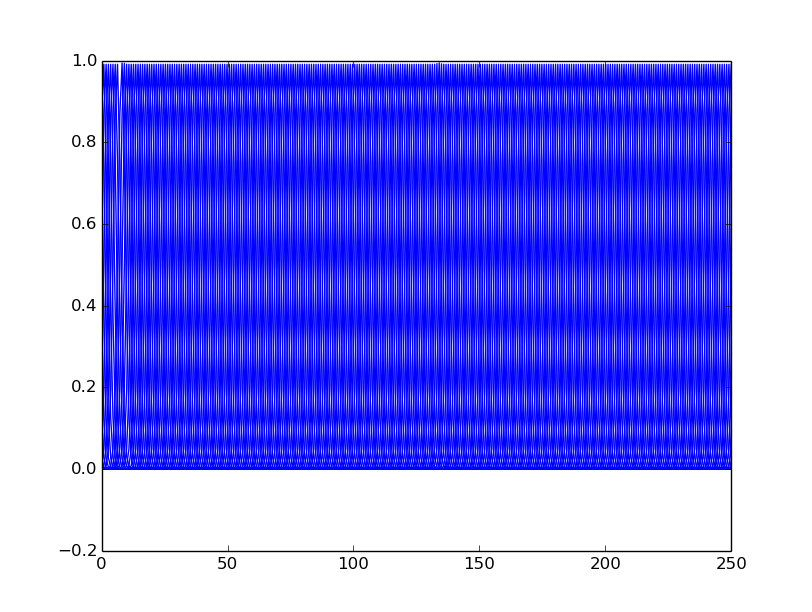
\includegraphics[scale=0.5]{die_welle6.png}\\
	\caption{for t=10}
\end{figure}\\
Nedenfor ses figurens to initialiserings tidpunkter, når bølgen er halvvejs og når bølgen når enden.
\begin{figure}[h!]
	\centering
	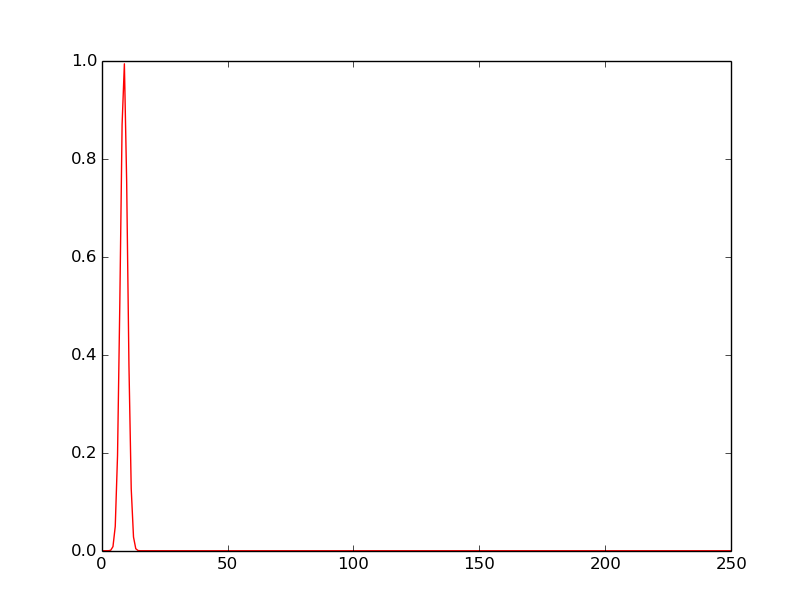
\includegraphics[scale=0.5]{die_welle8.png}\\
	\caption{for t=0}
\end{figure}\\
\begin{figure}[h!]
	\centering
	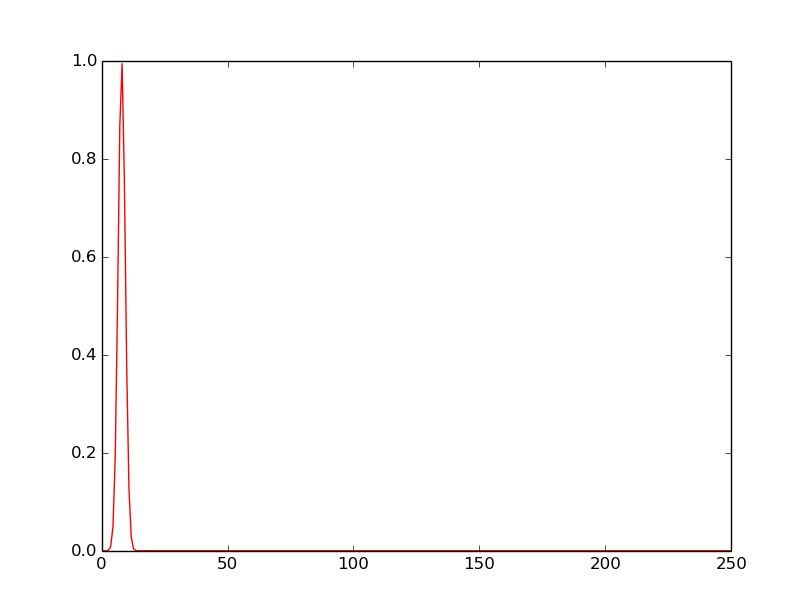
\includegraphics[scale=0.5]{die_welle9.png}\\
	\caption{til t=k}
\end{figure}
\end{document}